%% типы фазовых траекторий, а именно
% положение равновесия
% замкнутая траектория
% траектория без самопересечений
%% должны быть рассмотрены ранее

\subsection{Характер поведения фазовых траекторий в окрестности положения равновесия двумерной автономной нелинейной системы.}

Рассмотрим систему уравнений

\begin{equation}
  \begin{cases}
    \frac{d x}{d t} = f_1 (x, y) \\
    \frac{d y}{d t} = f_2 (x, y) \\
  \end{cases} 
\end{equation}

Пусть $M_0(x_0, y_0)$ -- положение равновесия данной системы, т. е. выполнено:
$\begin{cases}
  \frac{d x}{d t}(x_0, y_0) = 0 \\
  \frac{d y}{d t}(x_0, y_0) = 0
\end{cases}$

Для того, чтобы было проще исследовать фазовые траектории линеаризуем систему нелинейных автономных уравнений. Сделать это нам позволяет теорема \eqref{eq:linearisation} (дается без доказательства)

\begin{theorem} \label{eq:linearisation}
  Если линеаризация нелинейной системы в начале координат ($x = 0$) является простой автономной системой и $x = 0$ не является положением равновесия типа центр для исходной системы, то в окрестности $x = 0$ нелинейная система и ее линеаризация качественно эквивалентны.
\end{theorem}

Тогда, мы можем формально линеаризовать систему, используя известные методы (разложение до линейного члена):

\begin{equation}
  \begin{cases}
    \frac{d x}{d t} = \frac{\partial f_1}{\partial x} (x - x_0) + \frac{\partial f_1}{\partial y} (y - y_0) + o(\rho) \\
    \frac{d y}{d t} = \frac{\partial f_2}{\partial x} (x - x_0) + \frac{\partial f_2}{\partial y} (y - y_0) + o(\rho) \\        
  \end{cases}
\end{equation}

где $\rho = \sqrt{(x - x_0)^2 + (y - y_0)^2}$. В итоге, стандартной заменой $x = \overline{x} + x_0$ и $y = \overline{y} + y_0$ (переход в систему координат с центром в $(x_0, y_0)$) приводим систему к линейному виду.

\begin{equation}
  \begin{cases}
    \frac{d \overline{x}}{d t} = a_{11} \overline{x} + a_{12} \overline{y} \\
    \frac{d \overline{y}}{d t} = a_{21} \overline{x} + a_{22} \overline{y} \\        
  \end{cases}
\end{equation}

С этого момента, мы будем изучать виды фазовых траекторий и их поведение в окрестности положения равновесия для систем вида:

\begin{equation} \label{eq:base_system}
	\begin{cases}
		\frac{d x}{d t} = a_{11} x + a_{12} y \\
		\frac{d y}{d t} = a_{21} x + a_{22} y \\        
	\end{cases}
\end{equation}

с положением равновесия в точке $M_0(0, 0)$.

\subsection{Классификация положений равновесия линейной автономной системы второго порядка.}

Рассмотрим автономную однородную систему линейных ДУ \eqref{eq:base_system} и введем матрицу системы:

\begin{equation}
	A = 
	\begin{pmatrix}
		a_{11} ~~ a_{12} \\
		a_{21} ~~ a_{22} \\
	\end{pmatrix}
\end{equation}

Получим собственные значения этой матрицы:

\begin{equation}
	\begin{vmatrix}
		a_{11} - \lambda ~~ a_{12} \\
		a_{21} ~~ a_{22} - \lambda \\
	\end{vmatrix} = 
	\lambda^2 - \Tr A \cdot \lambda - \det A = 0 \Rightarrow
\end{equation}

\[ \lambda = \frac{\Tr A \pm \sqrt{\Tr^2 A - 4 \det A}}{2} \]

Фазовый портрет системы зависит от собственных значений матрицы $A$. Рассмотрим различные виды фазовых траекторий в зависимости от собственных значений.

\begin{enumerate}
  \item Собственные значения  $\lambda_1 \neq \lambda_2 \in \mathbb{R}$ (или $\Tr^2 A - 4 \det A > 0$)
  
  Тогда, в базисе собственных векторов матрица $A$ примет вид:
  $\overline{A} = 
  \begin{pmatrix}
    \lambda_1 ~~ 0 \\
    0 ~~ \lambda_2 \\
  \end{pmatrix}$

  система \eqref{eq:base_system} будет иметь вид:
  $\begin{cases}
    \frac{d x}{d t} = \lambda_1 x \\
    \frac{d y}{d t} = \lambda_2 y \\        
  \end{cases}$

  и решения данной системы в базисе собственных векторов:
  $\begin{cases}
    x(t) = c_1 e^{\lambda_1 t} \\
    y(t) = c_2 e^{\lambda_2 t} \\
  \end{cases}$

  Решение системы в исходном базисе:
  $
   \begin{pmatrix}
     x(t) \\
     y(t)
   \end{pmatrix} 
   = c_1 e^{\lambda_1 t} h_1 + c_2 e^{\lambda_2 t} h_2
  $,

  где $h_1, ~ h_2$ -- собственные векторы матрицы $A$.
  
  \textbf{Рассмотрим фазовые портреты}.
  
  \begin{enumerate}
  	\item $\lambda_1 < 0, ~~ \lambda_2 < 0$ и $|\lambda_1| < |\lambda_2|$
  	
  	Заметим прежде всего, что при $c_1 \neq 0, ~ c_2 = 0$ и при $c_1 = 0, ~ c_2 \neq 0$ мы получаем прямые линии с направляющими векторами $h_1$ и $h_2$. Поэтому векторы $h_1$ и $h_2$ являются решениями системы.
  	
  	Теперь, рассмотрим, что будет при $c_1 \neq 0$ и $c_2 \neq 0$. Из 
  	$\displaystyle 
  	\begin{cases}
  		x(t) = c_1 e^{\lambda_1 t} \\
  		y(t) = c_2 e^{\lambda_2 t} \\
  	\end{cases} \Rightarrow \\ 
  \Rightarrow t = \frac{1}{\lambda_1} \ln{\frac{x}{c_1}}$ подставляем в выражение для $y$ и получаем \textbf{в базисе собственных векторов} $\displaystyle y = c |x|^{\frac{\lambda_2}{\lambda_1}} = c |x|^r$, где $\displaystyle r = \frac{\lambda_2}{\lambda_1} > 0$.
  	
  	Таким образом мы приходим к выводу, что фазовые траектории в данном случае -- есть параболы (с показателем $r > 0$), причем при $t \rightarrow +\infty$ фазовые траектории стремятся \textbf{к} положению равновесия.

    \begin{definition}
    	Положение равновесия, при котором собственные значения матрицы $A$ одного знака и фазовые траектории направлены к положению равновесия называются \textbf{устойчивым узлом} рис \ref{fig:stable_node}.
    \end{definition}
    
    \begin{remark}
    	В случае, когда положение равновесия является узлом, фазовые траектории касаются оси с меньшим по модулю собственным числом.
    \end{remark}
    
    \begin{figure}[h!]
    	\begin{center}
    		\begin{minipage}[h!]{0.48\linewidth}
    			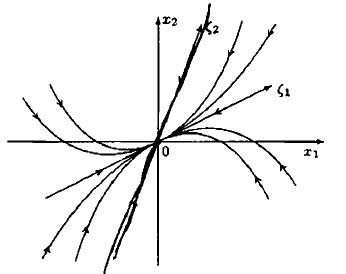
\includegraphics[width=1\linewidth]{stable_node.png}
    			\caption{Устойчивый узел, $\lambda_1, \lambda_2 < 0$}
    			\label{fig:stable_node}
    		\end{minipage}
    		\hfill
    		\begin{minipage}[h!]{0.48\linewidth}
    			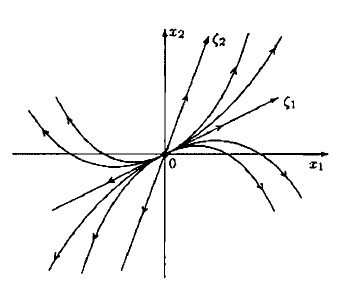
\includegraphics[width=1\linewidth]{unstable_node.png}
    			\caption{Неустойчивый узел $\lambda_1, \lambda_2 > 0$}
    			\label{fig:unstable_node}
    		\end{minipage}
    	\end{center}
    \end{figure}
    
    \item $\lambda_1 > 0, ~~ \lambda_2 > 0$ и $|\lambda_1| < |\lambda_2|$
    
    Расположение и вид траекторий (как и принцип их нахождения) остаются такими же, как и в первом случае, но направление движения по траекториям при $t \rightarrow +\infty$ меняется на противоположное.
    
    \begin{definition}
    	Положение равновесия, при котором собственные значения матрицы $A$ одного знака и фазовые траектории направлены от положения равновесия называются \textbf{неустойчивым узлом} рис \ref{fig:unstable_node}.
    \end{definition}
    
    \item $\lambda_1 < 0 < \lambda_2$
    
    В этом случае при $c_1 = c_2 = 0$ получаем положение равновесия $x = 0$, при $c_1 \neq 0, ~ c_2 = 0$ и при $c_1 = 0, ~ c_2 \neq 0$ мы получаем прямые линии с направляющими векторами $h_1$ и $h_2$. Для $c_1 \neq 0$ и $c_2 \neq 0$ аналогично первому случаю получим $\displaystyle y = c |x|^{\frac{\lambda_2}{\lambda_1}} = c |x|^r$, только в этом случае $\displaystyle r = \frac{\lambda_2}{\lambda_1} < 0$, поэтому траектории -- это кривые типа гиперболы. При этом оси с направляющими векторами $h_1$ и $h_2$ служат асимптотами траекторий типа гипербол и называются \textbf{сепаратрисами} \ref{fig:saddle}.
    
    \textbf{Положение равновесия в этом случае называется седлом системы}.
    
    \begin{figure}[h!]
    	\centering
    	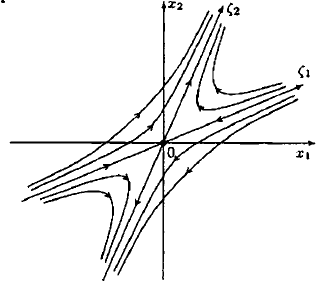
\includegraphics[scale=0.5]{saddle.png}
    	\caption{Седло $\lambda_1 < 0 < \lambda_2$}
    	\label{fig:saddle}
    \end{figure}

    \item $\lambda_1 = \lambda_2 = \lambda$, причем существует базис плоскости из собственных векторов $h_1$ и $h_2$ матрицы $A$.
    
    В этом случае решения системы в базисе собственных векторов:
    $\begin{cases}
    	x(t) = c_1 e^{\lambda t} \\
    	y(t) = c_2 e^{\lambda t} \\
    \end{cases}$
    каждое такое решение описывает в фазовой плоскости луч, выходящий из начала координат, причем движение по лучу при $t \rightarrow + \infty$ идет к нулю для $\lambda < 0$ и от нуля для $\lambda > 0$.
    
    При $\lambda < 0$ положение равновесия называется \textbf{устойчивым дикритическим (или звездным) узлом}, а при $\lambda > 0$ \textbf{неустойчивым дикритическим (или звездным) узлом} рис \ref{fig:stable_dicretic_node} и \ref{fig:unstable_dicretic_node}.

    \begin{figure}[h!]
      \begin{center}
          \begin{minipage}[h!]{0.48\linewidth}
              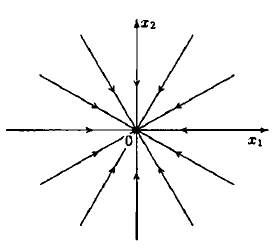
\includegraphics[width=1\linewidth]{stable_dicretic_node.png}
              \caption{Устойчивый дикритический узел, $\lambda < 0$}
              \label{fig:stable_dicretic_node}
          \end{minipage}
          \hfill
          \begin{minipage}[h!]{0.48\linewidth}
              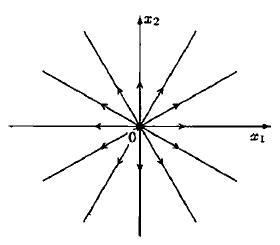
\includegraphics[width=1\linewidth]{unstable_dicretic_node.png}
              \caption{Неустойчивый дикритический узел $\lambda > 0$}
              \label{fig:unstable_dicretic_node}
          \end{minipage}
      \end{center}
    \end{figure}

    \item $\lambda_1 = \lambda_2 = \lambda$, причем существует базис плоскости из собственного вектора $h_1$ и присоединенного к нему вектора $h_2$ матрицы $A$.
    
    В этом случае
    $\begin{cases}
      x(t) = (c_1 + c_2 t) e^{\lambda t} \\
      y(t) = c_2 e^{\lambda t} \\
    \end{cases}$

    Из этой системы видно, что прямая с направляющим собственным вектором будет являться решением, а прямая с направляющим присоединенным вектором решением являться не будет.
    
    Подобные фазовые траектории называются устойчивыми и неустойчивыми вырожденными узлами рис \ref{fig:stable_degenerate_node} и \ref{fig:unstable_degenerate_node}.

    \begin{figure}[h!]
    	\begin{center}
    		\begin{minipage}[h!]{0.48\linewidth}
    			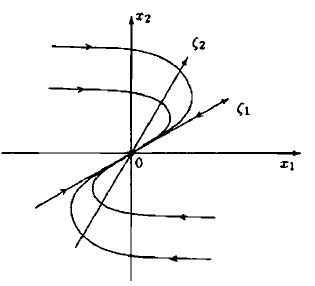
\includegraphics[width=1\linewidth]{stable_degenerate_node.png}
    			\caption{Устойчивый вырожденный узел, $\lambda < 0$}
    			\label{fig:stable_degenerate_node}
    		\end{minipage}
    		\hfill
    		\begin{minipage}[h!]{0.48\linewidth}
    			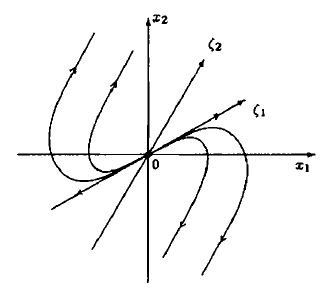
\includegraphics[width=1\linewidth]{unstable_degenerate_node.png}
    			\caption{Неустойчивый вырожденный узел $\lambda > 0$}
    			\label{fig:unstable_degenerate_node}
    		\end{minipage}
    	\end{center}
    \end{figure}
    
	\end{enumerate}
	
	\item Собственные значения  $\lambda_1, ~ \lambda_2 ~ \in ~ \mathbb{C}$ (или $\Tr^2 A - 4 \det A < 0$)
	
	В этом случае собственные значения матрица $A$ будут комплексными, запишем их в следующем виде:
	$\lambda_{1, 2} = r \pm i \omega$. Так же, запишем выражения для собственных векторов матрицы:
	$\vec{h}_{1, 2} = \vec{a} \pm i \vec{b}$. Тогда решение в базисе собственных векторов запишется в следующем виде:
  $\begin{cases}
  	x(t) = c e^{r t}(\cos (\omega t) + i \sin (\omega t)) \\
  	y(t) = \overline{c} e^{r t}(\cos (\omega t) - i \sin (\omega t)) \\
  \end{cases}$
  где $c, \overline{c} \in \mathbb{C}$. Выделим действительное решение. Один из способов выделения действительного решения: положим комплексные константы таковыми: $c = c_0 e^{i \varphi}$, $\overline{c} = c_0 e^{-i \varphi}$, где $c_0 \in \mathbb{R}$. Подставим константы в решение и получим:
  
  \begin{equation}
  	\begin{cases}
  		y(t) = c_0 e^{r t} e^{-i(\omega t + \varphi)} \\
  		x(t) = c_0 e^{r t} e^{i(\omega t + \varphi)} \\
  	\end{cases}
  \end{equation}
  
  это вид решения в базисе собственных векторов, перейдем обратно в исходный базис и получим:

  \begin{equation}
    \begin{pmatrix}
      x(t) \\
      y(t) \\
    \end{pmatrix} = c_0
    \begin{pmatrix}
      \vec{a} + i \vec{b} \\
      \vec{a} - i \vec{b} \\
    \end{pmatrix}
    e^{r t}
    \begin{pmatrix}
      e^{i(\omega t + \varphi)} \\
      e^{-i(\omega t + \varphi)} \\
    \end{pmatrix}
  \end{equation}

  отсюда несложно выразить:

  \begin{equation}
    \begin{pmatrix}
      x \\ 
      y \\
    \end{pmatrix} = 
    c_0 e^{r t} (2 \vec{a} \cos (\omega t + \varphi) - 2 \vec{b} \sin (\omega t + \varphi)),
  \end{equation}

  переходя к базису независимых векторов $\vec{a}$ и $\vec{b}$, получим:

  \begin{equation}
    \begin{cases}
      x = c_0 e^{r t} \cos {\chi} \\
      y = c_0 e^{r t} \sin {\chi}
    \end{cases}
  \end{equation}
  
  где $\chi = \omega t + \varphi$. Чтобы понять вид фазовой траектории перейдем к полярным координатам:

  \begin{equation}
    \begin{cases}
      \rho = c_0 e^{r \frac{\chi - \varphi}{\omega}} \\
      \chi = \omega t + \varphi \\
    \end{cases}
  \end{equation}

  рассмотрим полученные уравнения и выделим два принципиальных случая.

  \begin{enumerate}
    \item $r \neq 0$
    
    В этом случае видно, что фазовая траектория представляет собой спираль, причем если $r > 0$ спираль раскручивается, а если $r < 0$ -- закручивается. Такое положение равновесия называется \textbf{фокусом} рис \ref{fig:stable_fockus_a12gt0}, \ref{fig:stable_fockus_a12lt0}, \ref{fig:unstable_fockus_a12gt0}, \ref{fug:unstable_fockus_a12lt0}. Заметим, что направление закручивания (или раскручивания) определяется направлением фазовой скорости.

    \begin{figure}[h!]
      \begin{center}
          \begin{minipage}[h!]{0.48\linewidth}
              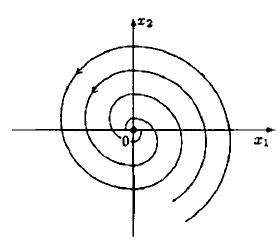
\includegraphics[width=1\linewidth]{stable_fockus_a12gt0.png}
              \caption{Устойчивый фокус}
              \label{fig:stable_fockus_a12gt0}
          \end{minipage}
          \hfill
          \begin{minipage}[h!]{0.48\linewidth}
              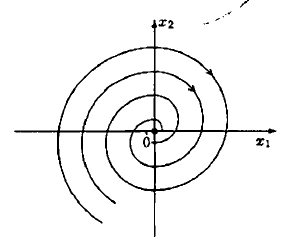
\includegraphics[width=1\linewidth]{stable_fockus_a12lt0.png}
              \caption{Устойчивый фокус}
              \label{fig:stable_fockus_a12lt0}
          \end{minipage}
          \hfill
          \begin{minipage}[h!]{0.48\linewidth}
              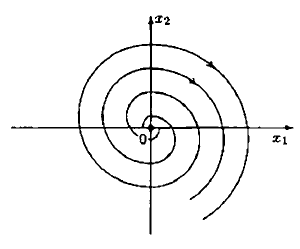
\includegraphics[width=1\linewidth]{unstable_fockus_a12gt0.png}
              \caption{Неустойчивый фокус}
              \label{fig:unstable_fockus_a12gt0}
          \end{minipage}
          \hfill
          \begin{minipage}[h!]{0.48\linewidth}
              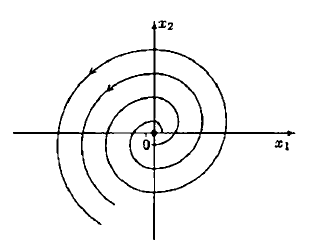
\includegraphics[width=1\linewidth]{unstable_fockus_a12lt0.png}
              \caption{Неустойчивый фокус}
              \label{fug:unstable_fockus_a12lt0}
          \end{minipage}
      \end{center}
  \end{figure}

  \item $r = 0$
  
  В этом случае в базисе векторов $\vec{a}$ и $\vec{b}$ фазовые траектории будут представлять собой окружности, что видно из уравнений 
  $
  \begin{cases}
    x = c \cos {\chi} \\
    y = c \sin {\chi}
  \end{cases}
  $ соответственно, в исходном базисе траекториями будут концентрические эллипсы. Подобное положение равновесия называется \textbf{центром системы} рис \ref{fig:center1}, \ref{fig:center2}.

  \begin{figure}[h!]
    \begin{center}
        \begin{minipage}[h!]{0.48\linewidth}
            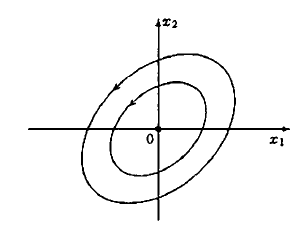
\includegraphics[width=1\linewidth]{center1.png}
            \caption{Центр системы}
            \label{fig:center1}
        \end{minipage}
        \hfill
        \begin{minipage}[h!]{0.48\linewidth}
            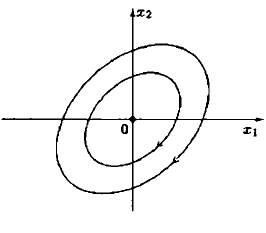
\includegraphics[width=1\linewidth]{center2.png}
            \caption{Центр системы}
            \label{fig:center2}
        \end{minipage}
    \end{center}
  \end{figure}

  \end{enumerate}

\end{enumerate}

\subsection{Теорема о выпрямлении траекторий}

Пусть точка $\vec x_0$ \textbf{не является особой точкой автономной системы} 

\begin{equation}
  \frac{d x_i}{d t} = f_i(\vec x)
\end{equation}

т. е. $f(\vec x_0) \neq \vec 0$, $\vec x_0 \in D \subset \mathbb{R}^n$, где $D$ -- область фазового пространства. 

Пусть при этом $\vec \varphi(t, \vec x_0)$ -- решение этой системы, такое, что $\vec \varphi(0) = \vec x_0$. В этом случае справедлива \textbf{теорема о выпрямлении} (дается без доказательства):

\begin{theorem}
  Существует окрестность точки $\vec x_0$, такая что в этой окрестности фазовая траектория с точностью до $o(t)$ является прямой линией с направляющим вектором $\vec{q} = \frac{\vec{f}(\vec x)}{|\vec f(\vec x)|}$.
\end{theorem}